\subsection{Первичная аутентификация в OpenID}
\selectlanguage{russian}

Из-за большого числа различных логинов, которые приходится использовать для доступа к разным сервисам, постепенно происходит внедрение единых систем аутентификации для разных сервисов (single sign-on), например, OpenID. Одновременно происходит концентрация пользователей вокруг больших порталов с единой аутентификацией, например, Google Account. Яндекс.Паспорт также уменьшает число используемых паролей для разных служб.

Принцип аутентификации состоит в следующем.
\begin{enumerate}
    \item Пользователи и интернет-сервисы доверяют аутентификацию третьей стороне -- центру единой аутентификации.
    \item Когда пользователь заходит на интернет-ресурс, веб-приложение перенаправляет его на центр аутентификации с защитой TLS-соединением.
    \item Центр аутентифицирует пользователя и выдаёт ему токен аутентификации, который пользователь предъявляет интернет-сервису.
    \item Сервис по токену аутентификации определяет имя пользователя.
\end{enumerate}

\begin{figure}[!ht]
	\centering
	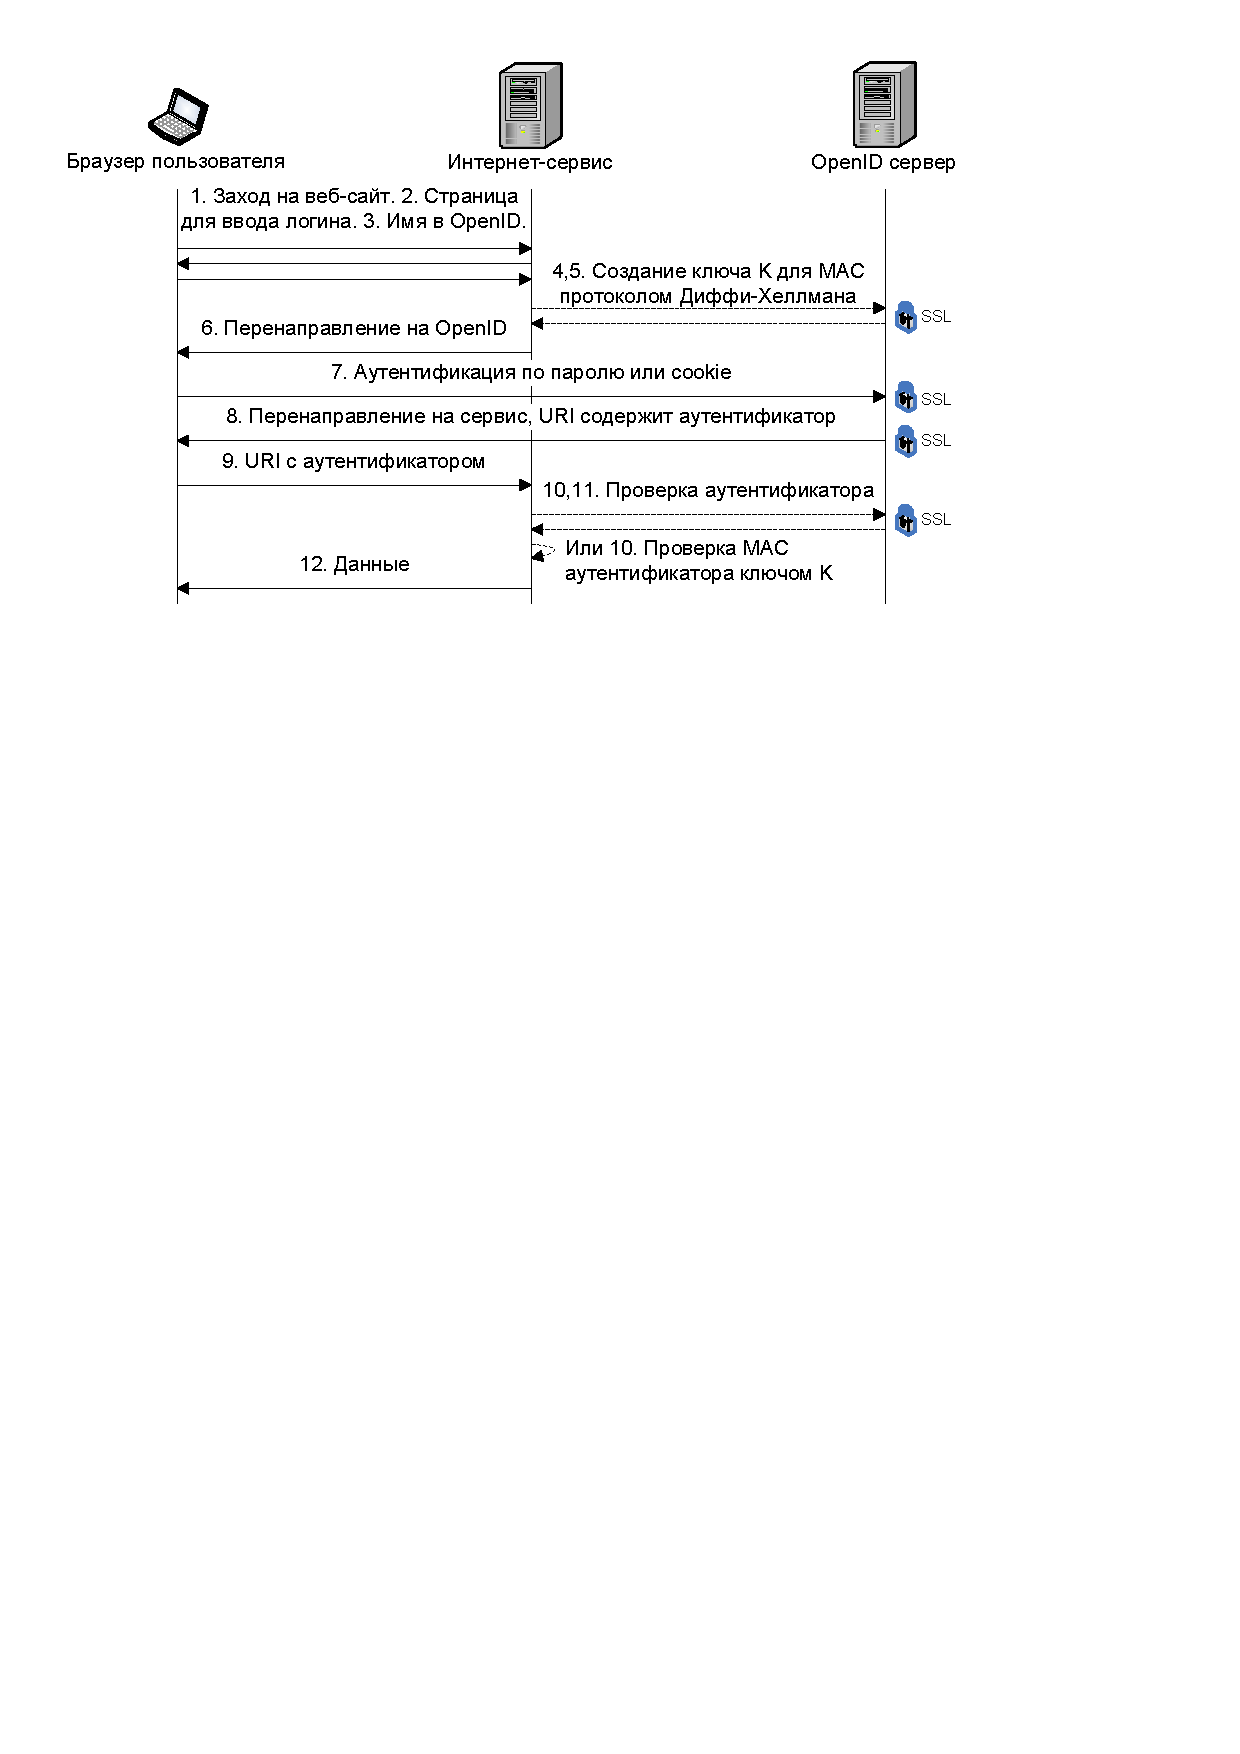
\includegraphics[width=0.9\textwidth]{pic/openid}
	\caption{Схема аутентификации в OpenID\label{fig:openid}}
\end{figure}

На рис.~\ref{fig:openid} показана схема аутентификации в OpenID версии 2 для доступа к стороннему интернет-сервису.

Если сервис и центр вместе создают общий секретный ключ $K$ для имитовставки\index{имитовставка} $\MAC_K$, выполняются шаги 4, 5 по протоколу Диффи~---~Хеллмана\index{протокол!Диффи~---~Хеллмана}:
\[ \begin{array}{l}
    \text{4. Сервис} ~\rightarrow~ \text{центр: модуль}~ p ~\text{группы}~ \Z_p^*, ~\text{генератор}~ g, \\
        ~~~~~~~~~~~~~~~\text{число}~ g^a \mod p, \\
    \text{5. Сервис} ~\leftarrow~ \text{центр: число}~ g^b \mod p, ~\text{гаммированный} \\
        ~~~~~~~~~~~~~~~\text{ключ}~ K \oplus (g^{ab} \mod p),
\end{array} \]
то аутентификатор содержит $\MAC_K$, проверяемый шагом 10, на выданном ключе $K$\footnote{Более правильным подходом является использование в качестве ключа $K = g^{ab} \mod p$, так как в этом случае ключ создаётся совместно, а не выдаётся центром.}. Имитовставка\index{имитовставка} определяется как описанный ранее $\HMAC$ с хэш-функцией SHA-256.

Если сервис и центр не создают общий ключ (этапы 4, 5 не выполняются), то сервис делает запрос на проверку аутентификатора в шагах 10, 11.

В OpenID аутентификатор состоит из следующих основных полей: имени пользователя, URL сервиса, результата аутентификации в OpenID, одноразовой метки и, возможно, кода аутентификации от полей аутентифкатора на секретном ключе $K$, если он был создан на этапах 4, 5. Одноразовая метка является \emph{одноразовым} псевдослучайным идентификатором результата аутентификации, который центр сохраняет в своей БД. По одноразовой метке сервис запрашивает центр о верности результата аутентификации на этапах 10, 11. Одноразовая метка дополнительно защищает от атак воспроизведения.

Можно было бы исключить шаги 4, 5, 10, 11, но тогда сервису бы пришлось реализовывать и хранить в БД использованные одноразовые метки для защиты от атак воспроизведения. Цель OpenID -- предоставить аутентификацию с минимальными издержками на интеграцию. Поэтому в OpenID реализуется модель, в которой сервис все проверки делегирует запросами к центру.

Важно отметить, что в аутентификации через OpenID необходимо использовать TLS-соединения\index{протокол!SSL/TLS} (то есть протокол HTTPS\index{протокол!HTTPS}) на всех взаимодействиях с центром, так как в самом протоколе OpenID не производится аутентификация сервиса и центра, конфиденциальность и целостность не поддерживаются.
